\chapter{Programming Languages and Linux commands}

Today's lecture will focus on programming languages and how to give a computer instructions through a command line. Programming languages allow programmers to write instructions that can be interpreted by a computer to perform operations. Computers can not understand programming languages directly, so they have to be translated to a format that the computer can understand. In Java that transformation is referred to as compilation. When Java code is compiled, a program called a compiler takes the Java code as input and as output produces code that’s easier for a computer to execute directly. \\

For instance, suppose that you have a text file with a large number of itemized expenses and you’d like to calculate the total of the expenses. Writing instructions for this task that the computer’s hardware could understand directly could take more time than summing the entire list manually. Using a programming language to specify the instructions allows you to efficiently tell the computer to perform this task. \\ 

\section{Most popular programming languages}

What programming languages are most used depends on the application that the programming language is best used for. Java is one of the most popular programming languages. It’s used extensively by large companies; it powers many of the services of companies like Oracle and Amazon. It’s also one of the primarily languages used to develop applications for the Android mobile operating system. \\

JavaScript is another very popular language. Despite its similarity to Java in name, it is a very different language from Java. It’s the primary language used for writing code to interact with browsers in websites. It powers features of websites like generating dynamic content, sending requests to a server, making sure that the information entered in forms is correct, and many more things. It’s also increasingly used to write applications. It’s a popular choice among newer and smaller companies. \\

The number and diversity of programming languages can be intimidating, but learning new programming languages languages becomes easier once you have a solid understanding of fundamental concepts. In this course we use one programming language, but the ideas and concepts you learn can help you learn any programming language you need to. We recommend focusing on one programming language initially to learn fundamental concepts rather than spending time trying to learn multiple languages. We’ve decided to focus on Java because it’s easier to learn, widely used, and illustrates many important concepts in programming. 40\% of developers who responded to a large survey of developers stated that they know Java! \\

\section{Overview of a GUI}

Using a graphical user interface (GUI) or command line are the two primary ways to interact with your computer and complete task like edit files, create folders, and run programs. A graphical user interface like a file explorer (see figure 7.1) provides an easy way for users to complete tasks on their computer. A graphical user interface is the primary way most users of a computer interact with the computer. It’s popular because users can use their mouse and intuitive commands to complete basic tasks. \\

\begin{figure}
	\centering
	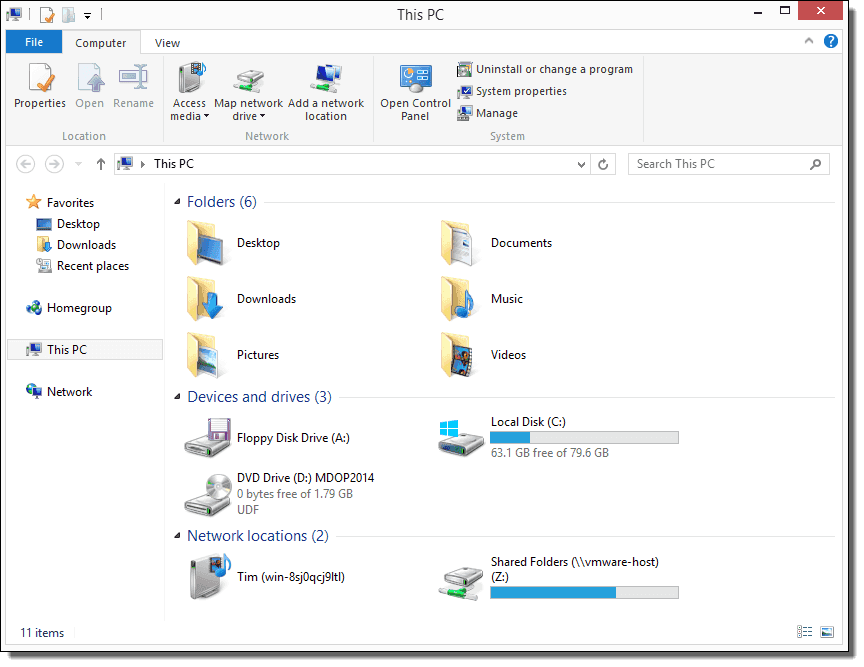
\includegraphics[width=0.85\textwidth]{images/windowsGUI.png}
	\caption{Windows file explorer}
	\label{fig:windows:file}
\end{figure}

The graphical user interface abstracts the details of the commands being issued to the computer away from the user of the program. This abstraction provides simplicity, but it also limits the flexibility of what a user can do with the computer. Furthermore, it means that users can only interact with a system that has a graphical user interface installed. This doesn’t include servers, computers without standard operating system, or computers that a user is connected to remotely. \\

The command line is a program you can access through the GUI of a linux machine. It’s also installed on servers without a GUI and can be accessed directly through monitors (this was the only way to interact with computers before the invention of the GUI).\\

A command line allows the user to issue a broader range of commands and interact with computers without a graphical user interface. It gives users the ability to interface directly with the operating system and issue commands that it can understand. This increases the range of the commands that the user can issue, giving them more flexibility to perform complex and custom tasks. \\

We will discuss the command line used in the Linux operating system because it is one of the most command and intuitive command lines. \\

\begin{center}
    \begin{tabular}{| l | p{75mm} | }
      \hline
      Command & Description \\ \hline
      ls & List all the files in the current directory \\ \hline
      touch & Create a new file \\ \hline
      cd [directory] & Changes the current directory to the directory given \\ \hline
      mkdir & Create a new directory within the current directory \\ \hline
      man [command] & Display the manual for a certain command \\ \hline
      cat [file] & Display the contents of file in the terminal \\ \hline
      mv [file] [location] & Moves files to a new location. \newline By default it moves file to a different name within the same directory. \\ \hline
      cp [file] [location] & Creates a new file with identical contents to the file specified in a new location. If a path for the file isn’t given, it will copy the file to the same directory. \\ \hline
    \end{tabular}
\end{center}
  
  A folder in Linux is referred to as a directory. When you open a command line, you’re in a certain directory within the file system. All commands that you issue that relate to interacting with the file system like creating files, editing files, or renaming files will be issued in the context of this directory. This is like navigating to a particular folder within the GUI file explorer and completing all your operations relative to that folder. 

\begin{figure}
	\centering
	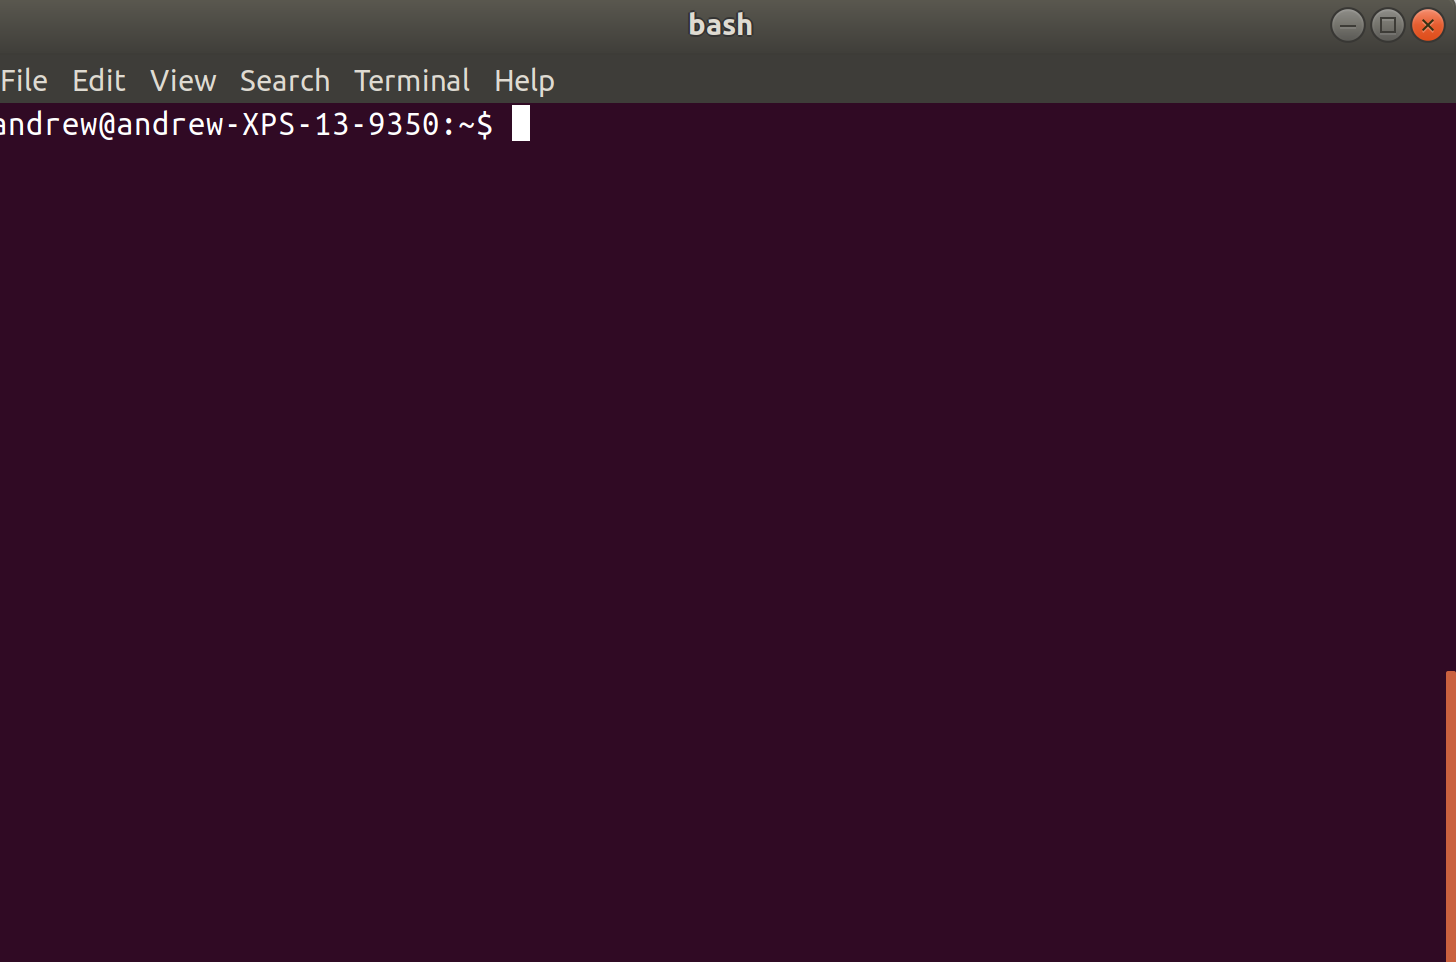
\includegraphics[width=0.85\textwidth]{images/commandLineOne.png}
	\caption{Linux command line}
	\label{fig:linux:one}
\end{figure}

Figure 7.2 shows the command line interface for a Linux computer. The prompt shown is where the user can type commands. By default it prepends the user’s name, the name of the computer, and a dollar sign. The white rectangle represents the location of my cursor prompting the user to enter commands. \\

To make a new directory, the user can use the ‘mkdir’ command. This is like making a new folder within an existing folder in the window’s file explorer. \\

To navigate to that directory the user can use the ‘cd’ command, short for change directory. Figure 7.3 displays an example of creating a new directory and changing to use that directory. In this example the ~ sign prepending the command represents the user’s home directory. The home directory is the outer most folder for that user’s account on the server or machine. \\

\begin{figure}
	\centering
	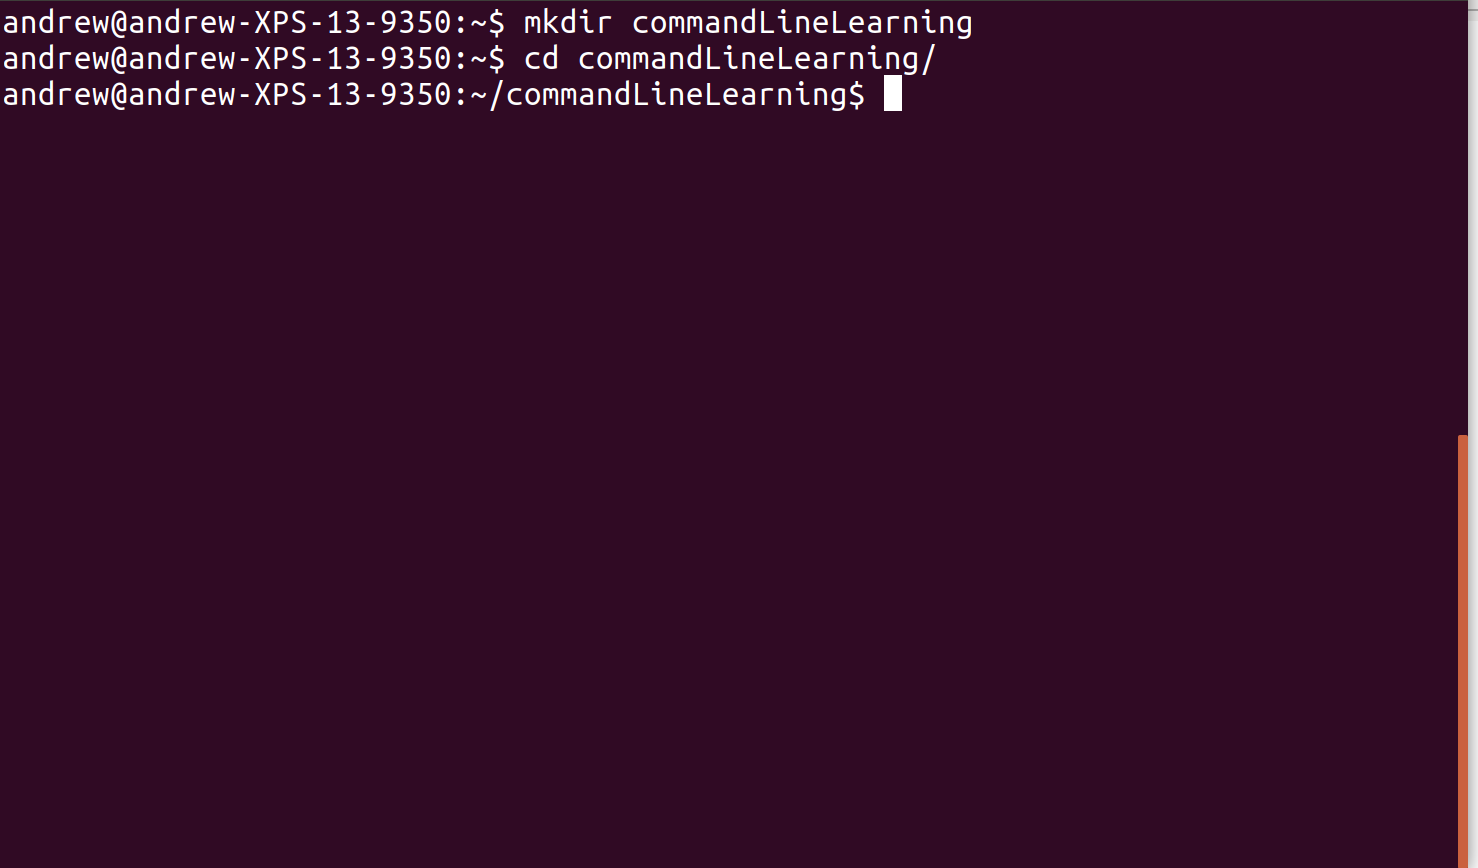
\includegraphics[width=0.85\textwidth]{images/commandLineTwo.png}
	\caption{Creating a directory}
	\label{fig:linux:two}
\end{figure}

\begin{figure}
	\centering
	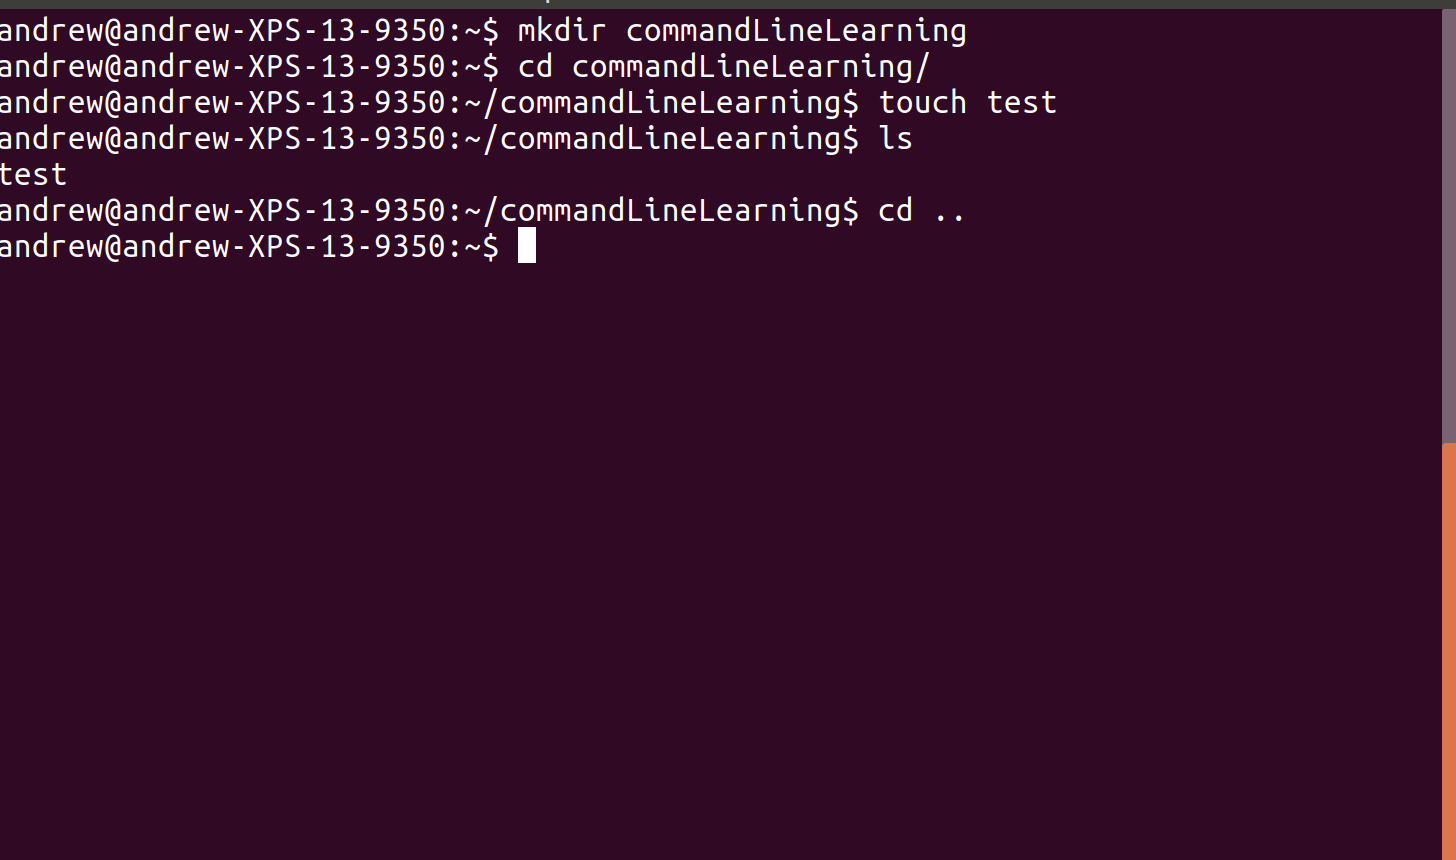
\includegraphics[width=0.85\textwidth]{images/commandLineThree.png}
	\caption{Listing files and navigating}
	\label{fig:linux:three}
\end{figure}

\begin{figure}[ht]
	\centering
	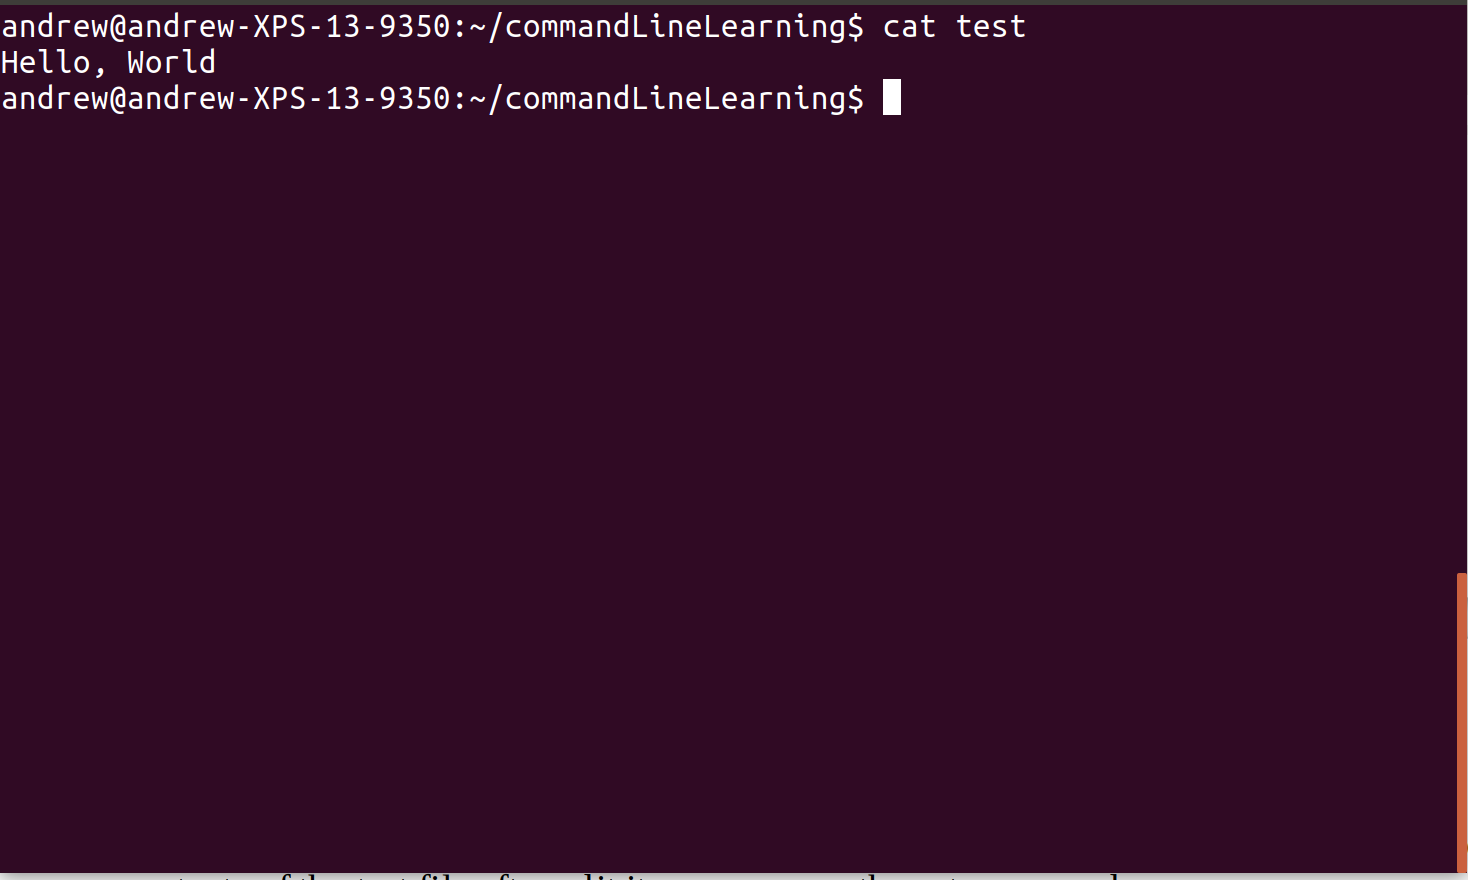
\includegraphics[width=0.85\textwidth]{images/commandLineFour.png}
	\caption{Cat command example}
	\label{fig:linux:four}
\end{figure}

In figure 7.3 I create a commandLineLearning directory and change my current directory to that directory. If I want to create a file in that directory, I can use the ‘touch’ command to create a new file. If I want to see the files in the directory, I can use the ‘ls’ command to list all of the files in the current directory. If I want to move back to the directory I was in before, I can use the ‘cd’ command with the parameters ‘..’ to move to the directory my current directory is contained within. In Linux, ‘..’ refers to the directory that contains your current directory, or the parent directory. These commands are summarized in figure 7.4. \\

Try these commands out. You can edit the contents of test using any file editing software. To view the contents of the test file after edit it, you can use the cat command. \\

\referencessection

Stack Overflow Developer Survey 2019. (n.d.).